\documentclass{article}
% \documentclass[preprint]{article}

% ready for submission
% \usepackage{neurips_2024}
\usepackage[preprint,nonatbib]{neurips_2024}

% \usepackage{graphicx}
% \usepackage[utf8]{inputenc} % allow utf-8 input
% \usepackage[T1]{fontenc}    % use 8-bit T1 fonts
% %\usepackage{hyperref}       % hyperlinks
% \usepackage{url}            % simple URL typesetting
% % \usepackage{booktabs}       % professional-quality tables
% \usepackage{amsfonts}       % blackboard math symbols
% \usepackage{nicefrac}       % compact symbols for 1/2, etc.
% \usepackage{microtype}      % microtypography
% \usepackage[utf8]{inputenc}
% % \usepackage{geometry}
% % \usepackage{graphics}
% \usepackage{multirow}
% \usepackage{rotating}
% % \usepackage[caption=false]{subfig}
% \usepackage{verbatim}
% % \usepackage{booktabs}
% \usepackage{array}
% \usepackage{textcomp, gensymb}
% \usepackage{diagbox}
% \usepackage[T1]{fontenc}    % use 8-bit T1 fonts
% \usepackage{url}            % simple URL typesetting
% % \usepackage{booktabs}       % professional-quality tables
% \usepackage{amsfonts}       % blackboard math symbols
% \usepackage{nicefrac}       % compact symbols for 1/2, etc.
% \usepackage{microtype}      % microtypography
% \usepackage{setspace}
% % \usepackage{geometry}
% % \usepackage{graphics}
% \usepackage{multirow}
% \usepackage{amssymb}
% \usepackage{diagbox}
% \usepackage{mathtools}
% \usepackage{wrapfig}
% \usepackage{diagbox} 
% \usepackage{wrapfig,lipsum,booktabs}
% \usepackage{caption}
% \usepackage{appendix}
% \usepackage{enumitem}

\usepackage[utf8]{inputenc} % allow utf-8 input
\usepackage[T1]{fontenc}    % use 8-bit T1 fonts
% \usepackage{hyperref}       % hyperlinks
\usepackage{url}            % simple URL typesetting
\usepackage{booktabs}       % professional-quality tables
\usepackage{amsfonts}       % blackboard math symbols
\usepackage{nicefrac}       % compact symbols for 1/2, etc.
\usepackage{microtype}      % microtypography
\usepackage{multirow}
\usepackage{graphics}
\usepackage{appendix}
\usepackage{graphicx}


\usepackage{color}
\usepackage[dvipsnames]{xcolor}
%\usepackage[table]{xcolor}
\definecolor{citecolor}{RGB}{0,113,188}
%\definecolor{citecolor}{HTML}{0071bc}
\usepackage{colortbl}
% \usepackage{booktabs} % For \hline and \shline (if defined)
\usepackage{amsmath} % For math and text formatting
\usepackage{pifont}% http://ctan.org/pkg/pifont
\usepackage{caption}

\usepackage[pagebackref=false,breaklinks=true,letterpaper=true,citecolor=citecolor,colorlinks,bookmarks=false]{hyperref}
% \usepackage{hyperref}
\definecolor{tblue}{RGB}{80,80,245}
\definecolor{tred}{RGB}{250,100,100}
\definecolor{golden}{RGB}{204,209,23}
\definecolor{green}{RGB}{15,108,16}
\newcommand{\hanwen}[1]{{\color{magenta}[hanwen: #1]}}
\newcommand{\SRnote}[1]{{\color{blue}[\textbf{SR}: #1]}}
\newcommand{\KGnote}[1]{{\color{red}[\textbf{KG}: #1]}}

\newcommand{\SR}[1]{{\color{black}#1}}
\newcommand{\KG}[1]{{\color{black}#1}}
\newcommand{\HJ}[1]{{\color{black}#1}}

\newcommand{\cc}[1]{{\color{cyan}#1}} % content to clear

\newcommand{\ve}[1]{\mathbf{#1}} % for displaying a vector
\newcommand{\ma}[1]{\mathrm{#1}} % for displaying a matrix

\newcolumntype{x}[1]{>{\centering\arraybackslash}p{#1pt}}

\newcommand{\bd}[1]{\textbf{#1}}
\newcommand{\app}{\raise.17ex\hbox{$\scriptstyle\sim$}}
\newcommand{\ncdot}{{\mkern 0mu\cdot\mkern 0mu}}
\def\x{$\times$}
\newcommand{\dt}[1]{\fontsize{8pt}{.1em}\selectfont \emph{#1}}
\newlength\savewidth\newcommand\shline{\noalign{\global\savewidth\arrayrulewidth
  \global\arrayrulewidth 1pt}\hline\noalign{\global\arrayrulewidth\savewidth}}
\newcommand{\tablestyle}[2]{\setlength{\tabcolsep}{#1}\renewcommand{\arraystretch}{#2}\centering\footnotesize}

\newcommand{\customfootnotetext}[2]{{% Group to localize change to footnote
  \renewcommand{\thefootnote}{#1}% Update footnote counter representation
  \footnotetext[0]{#2}}}% Print footnote text
\newcommand{\padcell}{\cellcolor{citecolor!10}}
\newcommand{\padcellred}{\cellcolor{red!10}}

\DeclareMathOperator*{\argmin}{arg\,min}

% \usepackage{amssymb}% http://ctan.org/pkg/amssymb
% \usepackage{pifont}% http://ctan.org/pkg/pifont

\newcommand{\cmark}{\color{green}\ding{51}}%
\newcommand{\xmark}{\color{red}\ding{55}}%

\definecolor{tgreen}{RGB}{32,178,170}
\newcommand{\green}[1]{{\color{tgreen}#1}}

\newcommand{\tablefirst}{\cellcolor{gray!20}}
\newcommand{\modelname}{CoFie}


\newcommand\todo[1]{\textcolor{red}{#1}}

\newcommand{\para}[1]{\noindent{\bf #1}}

\newcommand{\R}{\mathbb{R}}
\let \bs=\mathbf
\let \set=\mathcal

\def \transpose {\mathrm{T}}
\def \score {\mathit{score}}
\def \E {\mathbb{E}}
\def \Ep {\textup{E}}

% math equations that are widely used
\def \SigmaA {\Sigma_{2,n}(A)}
\def \SigmaLG {\Sigma_{1,m}(L^{\set{G}})}
\def \soIm   {(\bs{s}\otimes I_{m})}
\def \stoIm   {(\bs{s}^{T}\otimes I_{m})}
\def \UoIm   {(U \otimes I_{m})}
\def \UtoIm   {(U^{T} \otimes I_{m})}
\def \Ainverse {U(\Sigma_{2,n}(A) - \lambda_1(A))^{-1}U^{T}}

\def \bx {\mathbf{x}}
\def \bt {\mathbf{t}}

\def \mean {\textup{mean}}
\def \Diag {\mathrm{Diag}}
\def \diag {\mathrm{diag}}
\def \Cov  {\textup{Cov}}
\def \SDF  {\textup{SDF}}
\def \edge {\textup{edge}}
\def \EMD {\textup{EMD}}
\def \Chamfer {\textup{Chamfer}}
\def \robust {\textup{robust}}
\def \joint {\textup{joint}}
\def \graph {\textup{graph}}
\def \cons {\textup{cons}}
\def \data {\textup{data}}
\def \reg {\textup{reg}}
\def \appx{\textup{appx}}
\def \KL {\textup{KL}}
\def \val {\textup{val}}
\def \gtt{\textup{gt}}
\def \sample{\textup{sample}}
\def \reg {\textup{reg}}
\def \det {\mathrm{det}}
\def \good {\textup{good}}
\def \bad {\textup{bad}}
\def \hex {\textup{hex}}
\def \cur {\textup{c}}
\def \trace {\mathrm{Tr}}
\def \Pr {\mathrm{Pr}}
\def \objective {\mathit{obj}}
\def \area {\mathit{area}}
\def \domain {\set{D}}
\def \opt {\set{opt}}
\def \gt {\textup{gt}}
\def \row {\mathit{row}}
\def \Trace{\mathit{Trace}}
\def \inconsistent {\textup{Conflict}}
\def \unary {\mathit{unary}}
\def \median {\textup{median}}
\def \exclusive {\textup{exclusive}}
\def \saliency {\textup{saliency}}
\def \structure {\textup{t}}
\def \content {\textup{c}}
\def \style {\textup{s}}
\def \base {\textup{b}}
\def \offset {\textup{o}}
\def \affine {\textup{aff}}
\def \saliency {\textup{saliency}}
\def \flow {\mathit{flow}}
\def \adj {\mathit{adj}}
\def \gt {\mathit{gt}}
\def \RELU {\textup{RELU}}
\def \ReLU {\textup{ReLU}}
\def \noise {\mathit{noise}}
\def \init {\mathit{in}}
\def \path {\mathit{path}}
\def \map {\mathit{map}}
\def \match {\mathit{match}}
\def \shape {\textup{shape}}
\def \chamfer {\textup{chamfer}}
\def \sdp {\textup{sdp}}
\def \hexf {\textup{hex}}
\def \spectral {\textup{spectral}}
\def \quadf {\textup{quad}}
\def \consistency {\mathit{consistency}}
\def \induced {\mathit{indu}}
\def \composition {\mathit{compose}}
\def \minimize {\textup{minimize} }
\def \shift {\textup{shift}}
\def \maximize {\textup{maximize}}
\def \subjectto {\textup{subject to}}
\def \sS {\set{S}}
\newcommand{\OH}{\overline{H}}
\def \sT {\set{T}}
%\newcommand*{\qed}{\hfill\ensuremath{\square}}

\newtheorem{lem}{\textbf{Lemma}}
\newtheorem{proposition}{\textbf{Proposition}}
\newtheorem{theorem}{\textbf{Theorem}}
\newtheorem{corollary}{\textbf{Corollary}}
\newtheorem{assumption}{\textbf{Assumption}}
\newtheorem{example}{\textbf{Example}}
\newtheorem{definition}{\textbf{Definition}}
\newtheorem{remark}{\textbf{Remark}}

\let \set = \mathcal
\let \bs = \boldsymbol
\newcommand{\Var}{\textup{Var}}

%\renewcommand{\qed}{\hfill\blacksquare}
\newcommand{\qedwhite}{\hfill \ensuremath{\Box}}


\title{\textit{\modelname{}}: Learning Compact Neural Surface Representations with \underline{Co}ordinate \underline{Fie}lds}


\author{Hanwen Jiang\quad Haitao Yang\quad Georgios Pavlakos\quad Qixing Huang\\
 Department of Computer Science, The University of Texas at Austin
 \\{\tt\small \hspace{1mm}\{hwjiang,yanght,pavlakos,huangqx\}@cs.utexas.edu}\\
}

\begin{document}

\maketitle

\vspace{0.05in}

\begin{abstract}
    This paper introduces \modelname{}, a novel local geometry-aware neural surface representation. \modelname{} is motivated by the theoretical analysis of local SDFs with quadratic approximation. We find that local shapes are highly compressive in an aligned coordinate frame defined by the normal and tangent directions of local shapes. Accordingly, we introduce Coordinate Field, which is a composition of coordinate frames of all local shapes. The Coordinate Field is optimizable and is used to transform the local shapes from the world coordinate frame to the aligned shape coordinate frame. It largely reduces the complexity of local shapes and benefits the learning of MLP-based implicit representations. Moreover, we introduce quadratic layers into the MLP to enhance expressiveness concerning local shape geometry. \modelname{} is a generalizable surface representation. It is trained on a curated set of 3D shapes and works on novel shape instances during testing. When using the same amount of parameters with prior works, CoFie reduces the shape error by $48\%$ and $56\%$ on novel instances of both training and unseen shape categories. Moreover, \modelname{} demonstrates comparable performance to prior works when using only $70\%$ fewer parameters. Code and model can be found here: \href{https://hwjiang1510.github.io/CoFie/}{https://hwjiang1510.github.io/CoFie/}
\end{abstract}

\vspace{0.05in}

\section{Introduction}
\label{sec:intro}
Deep neural networks (DNNs) have made remarkable progress across various domains by delivering superior performance on large-scale datasets. However, while the benefits of training DNNs on large-scale datasets are undeniable, these algorithms also tend to inadvertently acquire unwanted biases \cite{NEURIPS2020_6cfe0e61}, hampering their generalization. For instance, a classifier predominantly trained to recognize camels in desert landscapes could encounter difficulties when attempting to identify a camel situated on a road \cite{Kim_2021_ICCV}. While a certain degree of bias can enhance model performance, as exemplified by the assumption that cars usually travel on roads \cite{Choi_2020_CVPR}, it remains critical to identify and address unwanted biases. 
% \begin{figure}
%     \centering
%     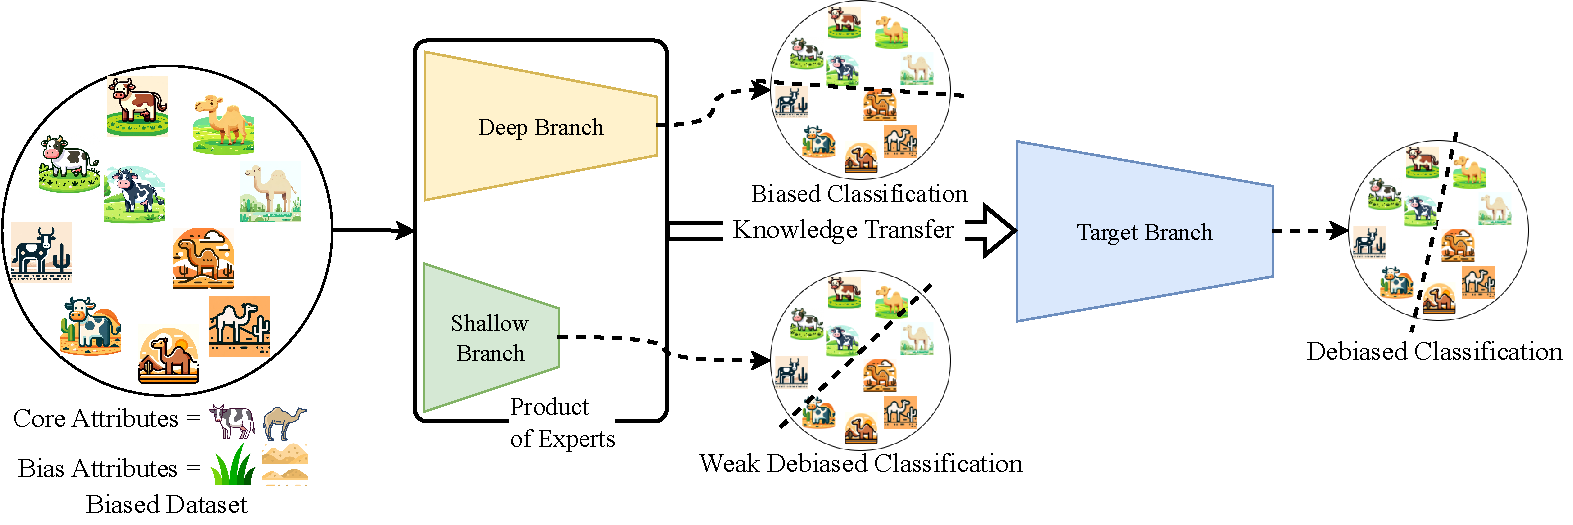
\includegraphics[width=\textwidth]{figures/teaser_diagram.pdf}
%     \caption{Our DeNetDM model comprises a Product of Expert (PoE) \cite{Hinton:02}, featuring one deep and one shallow expert. The shallow expert primarily captures core attributes, achieving debiased classification, while the deep expert focuses on bias. To compensate for the shallow expert's limited capability due to less depth, we implement a knowledge transfer strategy utilizing knowledge from the experts to train a target debiased model.}
%     \label{fig:teaser-diagram}
% \end{figure}
Previous methods to address this problem rely on bias annotations as suggested in \cite{9607491,Kim_2019_CVPR,sagawa2019distributionally,wang2020fair}, and may involve predefined bias types, such as texture bias mitigation approach in \cite{geirhos2018imagenettrained}. 
% . For instance, in \cite{geirhos2018imagenettrained}, texture bias is mitigated by training a shape-oriented classifier using augmented data and style transfer. However, this approach limits the ability of models to achieve robustness against biases for which obtaining prior knowledge is a challenging endeavor. 
However, acquiring bias labels with human resources is expensive and time-consuming. Recent studies, including \cite{NEURIPS2020_eddc3427} and \cite{NEURIPS2021_disentangled},  have shifted towards debiasing methods without bias labels, with approaches like \cite{NEURIPS2020_eddc3427} emphasizing bias-aligned samples and reweighting bias-conflicting samples, while others like \cite{NEURIPS2021_disentangled,Kim_2021_ICCV} introduce augmentation strategies to diversify bias-conflicting points.

We propose DeNetDM (\textbf{De}biasing by \textbf{Net}work \textbf{D}epth \textbf{M}odulation), a novel approach to automatically identify and mitigate spurious correlations in image classifiers without relying on explicit data augmentation or reweighting. We start by showing that a sample set that exhibits bias through spurious correlation of attributes lies on a manifold with an effective dimensionality (rank) lower than its bias-free counterpart.
% We then leverage this finding to formally derive a relationship between the depth of a network and the true rank of the attribute (not sample) subspace that it learns and generalizes to.
We then leverage this finding to formally derive a relationship between the depth of a network and the true rank of the attribute (not sample) subspace that it encodes. We find for a set of attributes that are equally likely to minimize the empirical risk, a deeper network prefers to retain those with a lower rank, with a higher probability. This implies that the depth of a network acts as an implicit regularizer in the rank space of the attributes.
We find that deeper networks tend to generalize based on bias attributes and shallower networks tend to generalize based on core attributes. This finding is in line with a number of works that show that deeper networks tend to learn low rank solutions in general \citep{roy2007effrank, huh2023simplicitybias, wang2024implicit}.
% Note, however, that previous works make no claim about the relationship between the depth of a network and the attribute subspace that it generalizes to, a link we establish in our work for the first time, to the best of our knowledge.
Note, however that prior works do not establish the relationship between network depth and the rank of the attribute subspace, a link we establish in our work for the first time, to the best of our knowledge.

Our theoretical claims are confirmed by our preliminary empirical study on linear feature decodability, which quantifies the extent to which specific data attributes can be accurately and reliably extracted from a given dataset or signal. Our study focuses on the feature decodability of bias and core attributes in the neural networks of varying depths, following the approach outlined in \cite{NEURIPS2020_71e9c662}. Our observations in untrained neural networks reveal that the feature decodability tends to diminish as the networks become deeper. We also investigate how attribute decodability varies with Empirical Risk Minimization (ERM) based training on networks of varying depths. 
% A detailed discussion of the experiment can be found in \cref{sec:linear_decodability_analysis}.


% DeNetDM is based on insights gained from our preliminary study on feature decodability, which quantifies the extent to which specific data attributes can be accurately and reliably extracted from a given dataset or signal. Our study focuses on the feature decodability of bias and core attributes in the neural networks of varying depths, following the approach outlined in \cite{NEURIPS2020_71e9c662}. Our observations in untrained neural networks reveal that the feature decodability tends to diminish as the networks become deeper. We also investigate how attribute decodability varies with Empirical Risk Minimization (ERM) based training on networks of varying depths. A detailed discussion of the experiment can be found in \cref{sec:linear_decodability_analysis}.
% We conduct a brief experiment to analyze the feature decodability, specifically focusing on bias and core attributes, using untrained neural networks of different depths, following the approach outlined in \cite{NEURIPS2020_71e9c662}. Our observations reveal that the attribute decodability tends to diminish as the neural networks becomes deeper. Additionally, we investigate the variation in attribute decodability when employing Empirical Risk Minimization (ERM) based training on networks of different depths. These experiments yield interesting results that form the foundation of our proposed approach DeNetDM. A detailed discussion of the experimental setting and the conclusions can be found in \cref{sec:linear_decodability_analysis}. 
% We eliminate the necessity for explicit reweighting or augmentation of bias-conflicting data points by employing a novel approach based on a simple observation, which entails modulating the depth of a pair of neural networks.

% \abhra{
% SUGGESTED REWRITE FOR THE LAST PARAGRAPH:
% We start by showing that a sample set that exhibits bias through spurious correlation of attributes lies on a manifold with an effective dimensionality (rank) lower than its bias-free counterpart. We then leverage this finding to formally derive a relationship between the depth of a network and the true rank of the attribute (not sample) subspace that it learns and generalizes to. We find that deeper networks tend to generalize based on bias attributes and shallower networks tend to generalize based on core attributes. This finding is in line with a number works that show that deeper networks tend to learn low rank solutions in general \citep{roy2007effrank, huh2023simplicitybias, wang2024implicit}. Note, however, that previous works make no claim about the relationship between the depth of a network and the attribute subspace that it generalizes to, a link we establish in our work for the first time, to the best of our knowledge.
% }
Our hypothesis posits that in a task requiring deep and shallow branches to acquire distinct information, the deep branch consistently prioritizes bias attributes, while the shallow branch favors core attributes. We utilize a technique inspired by the Product of Experts \citep{Hinton:02}, where one expert is deeper than the other. Empirical analysis shows that the deep branch becomes perfectly biased and the shallow branch becomes relatively debiased by focusing solely on the core attributes by the end of the training. Since the shallow branch may lack the capacity to capture the nuances of the core attributes adequately due to less depth, we propose a strategy where we train a deep debiased model utilizing the information acquired from both deep (perfectly biased) and shallow (weak debiased) network in the previous phase. Our training paradigm efficiently facilitates the learning of core attributes from bias-conflicting data points to the debiased model of any desired architecture. 

In summary, we make the following contributions: (1) We theoretically prove that the deep models prefer to learn spurious correlations compared to shallower ones, supported by empirical analysis of the decodability of bias and core attributes across neural networks of varying depths. (2) Building upon the insights from our decodability experiments, we present a novel debiasing approach that involves training both deep and shallow networks to obtain a desired debiased model. (3) We perform extensive experiments and ablation studies on a diverse set of datasets, including synthetic datasets like Colored MNIST and Corrupted CIFAR-10, as well as real-world datasets, Biased FFHQ, BAR and CelebA, demonstrating an approximate 5\% improvement over existing methods.
    % \item Our results demonstrate that our approach outperforms existing state-of-the-art methods, with an approximate 5\% performance improvement.



\section{Related Work}

% We discuss related work from three perspectives, namely implicit shape representations (Section~\ref{Subsec:Implicit:Shape:Rep}),  hybrid 3D representations (Section~\ref{Subsec:Hybrid:3D:Rep}), and coordinate field optimization (Section~\ref{Subsec:Coordinate:Field:Opt}).

%\vspace{-0.05in}
\noindent\textbf{Implicit Shape Representations.}
Implicit shape representations are state-of-the-art in encoding shape geometric details~\cite{DBLP:conf/cvpr/ParkFSNL19, DBLP:conf/nips/TancikSMFRSRBN20, DBLP:conf/nips/SitzmannMBLW20, aumentado2022representing, shen2021tetrahedra, yenamandra2024fire, wang2023neuralhessian}. 
To improve the shape modeling capability, researchers inject local-aware designs. For example, DeepLS~\cite{DBLP:conf/eccv/ChabraLISSLN20} integrates voxel grids and local MLPs to decode geometric shapes. Another line of work explores hierarchical representations where the local surfaces are divided unevenly~\cite{10.1145/882262.882293, wang2018adaptive, liu2021octsurf, tang2021octfield, 10.1145/3528223.3530087, takikawa2021nglod}, leveraging Octree. For example, Multilevel Partition of Pnity~\cite{10.1145/882262.882293} (MPU) blends parametric implicit surface patches into a global implicit surface. DOGNet uses dual-octree designs for neural MPU. 
The contribution of \modelname{} is perpendicular to these methods. \modelname{} still works on evenly divided voxels. However, instead of resolving high-frequency details of local shapes by using higher local resolution, \modelname{} proposes the Coordinate Field to reduce the spatial complexity. This is motivated by the analysis result that local geometric shapes are highly compressive under suitable coordinate frames. 


The idea of a coordinate field is related to several existing approaches. For example, MVP~\cite{10.1145/3450626.3459863} introduced oriented boxes for 3D face synthesis. However, in our setting, the variations in geometry and topology are much more significant than those of 3D human faces. 
Another relevant work is LDIF~\cite{DBLP:conf/cvpr/JiangSMHNF20}, which transforms a 3D point in the local coordinate system of each primitive to decode the iso-value of each shape. However, LDIF uses a fixed coordinate frame for each primitive. In contrast, the coordinate field varies spatially in \modelname{} and can be optimized, allowing us to capture detailed variations of the parts flexibly.
Moreover, \modelname{} is based on a rigorous analysis of the expressivity of SDF and SDF learning. A follow-up approach~\cite{DBLP:conf/cvpr/Zheng0DL21} uses a warping field to transform a 3D point into a canonical space of specific categories. In contrast, \modelname{} is category-agnostic, benefiting from the use of local shapes.


On the learning side, many approaches show that MLPs are expressive and that their performance depends on the loss of training. For example, SAL~\cite{DBLP:conf/cvpr/AtzmonL20} and SALD~\cite{DBLP:conf/iclr/AtzmonL21} show the importance of integrating normal losses to capture geometric features. SIREN~\cite{DBLP:conf/nips/SitzmannMBLW20} introduced other regularization losses to improve the quality of implicit representations learned. Although these approaches focus on local shape details, \modelname{} focuses on network design using coordinate frames. The \modelname{} approach is orthogonal to the encoding schemes. 

%\vspace{-0.05in}
\noindent\textbf{Hybrid 3D Representations.} Each 3D representation has fundamental advantages and limitations from the machine learning and representation perspective. For example, implicit representations allow flexible topologies, whereas explicit representations are easier to edit. Therefore, hybrid 3D representations, which aim to add the strength of different 3D representations for representation learning, have received a lot of attention. The main stream in hybrid 3D representations sequentially applies hybrid 3D models~\cite{10.1145/3072959.3073637, 10.1145/3526212, DBLP:conf/iccv/Gkioxari0M19, 10.1145/3355089.3356488, DBLP:conf/nips/ShenGYLF21}. For example, GRASS~\cite{10.1145/3072959.3073637} combines a part-based representation to capture geometric structures of 3D shapes and a volumetric representation per part to capture geometric details of the parts. DSG-Net~\cite{10.1145/3526212} employs part-based deformations to capture geometric details of the part. Other examples~\cite{DBLP:conf/iccv/Gkioxari0M19, 10.1145/3355089.3356488, DBLP:conf/nips/ShenGYLF21, DBLP:conf/eccv/ChabraLISSLN20, hong2023lrm, chan2022efficient, jiang2022few, jiang2023leap} combine explicit graph, mesh, voxel and triplane representations with implicit volumetric representations to encode geometry details. \modelname{} is relevant to this series of approaches, where it combines voxel grids to encode global shapes and an implicit representation to decode local geometric details. The novelty of \modelname{} is that the local module employs a coordinate frame representation and enforces the prior knowledge that the local shape is roughly a low-complexity polynomial surface in the coordinate system defined by normal and principal directions. 


\noindent\textbf{Coordinate Field Optimization.} The task of computing the proposed cell-based coordinate field is related to the problem of vector-field and frame-field design on meshes, where we want to ensure that the coordinate field is smooth and consistent among adjacent cells, and where we want the normal and tangent directions of each coordinate frame to align with the local fitting results if the fitting results are highly confident. This problem was studied in~\cite{10.1145/1183287.1183297}, which introduced a global optimization framework to compute a global vector field on a triangular mesh. Several more recent approaches have developed improved formulations for vector field optimization~\cite{10.1145/2816795.2818078,10.1145/2461912.2462005} and extensions to frame field optimization~\cite{10.1145/2601097.2601179,10.1145/2980179.2982408}. We refer to \cite{10.1145/3084873.3084921} for surveys on this topic. Rather than solving a global optimization problem to compute the coordinate field, the learning of the coordinate field in \modelname{} is driven by learning a compressive MLP. 
%We also introduce a novel loss to address uncertain principal directions and recover suitable orientations of principal directions. 




\section{Analysis of Fitting SDFs of Local Patches}
In this section, we provide an analysis of fitting local surfaces. Following prior works~\cite{Ohtake2003MultilevelPO, xiong2014shading, erens1993perception, wallace1981three}, we simplify local surfaces as quadratic patches. Additionally, we note that some works approximate local surfaces with linear patches~\cite{kolluri2008provably, wang2018adaptive}. However, to handle the geometry details, it usually requires extremely high~\cite{wang2018adaptive} or infinite resolution~\cite{kolluri2008provably} during local surface partition. Approximating local surfaces with quadratic patch is more practival.


\subsection{Importance of Non-linearity}
\label{sec: motivation_quadratic_mlp}

A quadratic surface patch can be represented by $\bs{f}(u,v) = (u,v, \frac{1}{2}(a u^2 + c v^2 + 2b uv))$, where $u^2 + v^2 \leq r^2$ for locality, and $a,b,c$ are parameters for controlling the shape of the quadratic patch. The following proposition characterizes the SDF of a point $\bs{p}$ to $\bs{f}$.

\begin{proposition}
For each point $\bs{p} = (x,y,z)^T$ in the neighborhood of the origin $\bs{o}$, the signed distance function from $\bs{p}$ to $\bs{f}(u,v)$ can be approximated as
\begin{equation}
d(\bs{p}, \bs{f}(u,v)) \approx z - \frac{1}{2}(a x^2 + c y^2 + 2b xy).
\label{SDF:Approx}   
\end{equation}
where the approximation omits third-and-higher order terms in $x$, $y$, and $z$.
\label{Prop:SDF:Approx}
\end{proposition}

\noindent\textsl{Proof:} See Appendix~\ref{Proof:Prop:SDF:Approx}.

Prop.~\ref{SDF:Approx} suggests that the SDF is non-linear. However, a shallow MLP using ReLU activation is piecewise linear, where the ReLU activation functions essentially decompose the input space into subspaces and the function in each subspace is still linear. This motivates the use of quadratic layers instead of linear layers (Sec.~\ref{sec: MLP}).

To hold generality, in Appendix~\ref{Proof:Prop:SDF:Approx2}, we also analyze the local surface that can not be simplified as a single quadratic patch, i.e. sharp edges as the intersection of two quadratic patches.


\subsection{Difficulty of Fitting Transformation Information}
\label{sec: difficaulty}
We demonstrate the difficulty of recovering the transformation information of quadratic patches during geometry fitting.


\noindent\textbf{Aligned Quadratic Patches.} Same as the previous section, we define the SDF of a quadratic local patch as $z - \frac{1}{2}(ax^2 + cy^2 + 2bxy)$, where the quadratic patch is axis-aligned. Consider a set of samples $\{((x_i,y_i,z_i), d_i),1\leq i \leq n\}$ from this quadratic patch, where $(x_i,y_i,z_i)$ is the location of the point $\bs{p}_i$, $d_i$ is the SDF value, and $n$ is the number of samples. To fit the surface from the samples, we solve the optimization problem as 
\begin{equation}
\argmin_{a,b,c} \sum\limits_{i=1}^n \big(z_i - \frac{1}{2}(ax_i^2 + cy_i^2 + 2bx_iy_i)-d_i\big)^2    
\end{equation}
which is a convex problem that has a unique global optimal. 

\noindent\textbf{Unaligned Quadratic Patches.}
Consider transforming the quadratic patch with a random rigid transformation $(R,\bs{t})$. This quadratic patch is not axis-aligned. In this case, the SDF function is given by $z'-\frac{1}{2}(a{x'}^2 + c{y'}^2 + 2bx'y')$ where $(x',y',z') = R(x,y,z) + \bs{t}$. To fit the surface from the samples, we solve the optimization problem as 
\begin{equation}
\argmin_{a,b,c,R,\bs{t}} \sum\limits_{i=1}^n \big(z_i' - \frac{1}{2}(a{x_i'}^2 + c{y_i'}^2 + 2b{x_i'}{y_i'})-d_i\big)^2, \quad \left( 
\begin{array}{c}
x_i' \\
y_i' \\
z_i'
\end{array}
\right)= R\left( \begin{array}{c}
x_i \\
y_i \\
z_i
\end{array}\right) + \bs{t}.
\label{Eq:Non:Convex}
\end{equation}

In this case, (\ref{Eq:Non:Convex}) becomes non-convex and has local minima. We defer a detailed characterization of the local minima of (\ref{Eq:Non:Convex}) to Appendix~\ref{Analysis:Non:Convex}. 

In general, this non-convex problem makes geometry fitting non-trivial. It motivates the use of the Coordinate Field to explicitly model the transformation information and disentangle the transformation information of local patches from its geometry (Sec.~\ref{sec: representation}).








\section{\modelname{}}
In this section, we introduce details of \modelname{}, including its representation (Sec.~\ref{sec: representation}), MLP architecture (Sec.~\ref{sec: MLP}), and its learning scheme (Sec.~\ref{sec: loss}).


\subsection{\modelname{} Representation}
\label{sec: representation}
As shown in Fig.~\ref{Fig:Overview}, \modelname{} is based on a \textit{hierarchical} representation, with coarse and fine-grained geometry. At the coarse level, it represents a shape with voxels. In detail, for a shape $\mathbf{S}$, it divides the space that contains the shape into $V\times V\times V$ non-overlapping voxel grids, where $V$ is the resolution of the voxel grids. A subset of voxels that intersect with the shape surface will be valid. 

At the fine-grained level, for each valid voxel $v$, we use an implicit representation to encode the geometry details for the local surface inside the voxel. Specifically, we use MLP-based neural SDFs. Each voxel $v$ has a latent code $z_v$ representing the local geometry and we use the MLP $g^{\theta}$ to decode the SDF values. For a point $\bs{x}$, its SDF value contributed by the voxel $v$ is
\begin{equation}
f(\bs{x},v) = g^{\theta}(\bs{x}_v, \bs{z}_v), \qquad \bs{x}_v = (\bs{n}_v, \bs{t}_v, \bs{n}_v\times \bs{t}_v)^T(\bs{x} - \bs{o}_v),
\end{equation}
where $(\bs{o}_{v},\bs{n}_v, \bs{t}_{v})$ parameterize the coordinate frame of voxel $v$. Ideally, $\bs{o}_{v}$, $\bs{n}_v$ and $\bs{t}_{v}$ are the origin, normal direction, and tangent direction of the local surface, respectively. 

Intuitively, for decoding the SDF value, we transform the point from the world coordinate system to the shared coordinate system for all local surfaces. $\bs{o}_{v}$ forms the translation between the two coordinate system, and $(\bs{n}_v, \bs{t}_{v})$ form the rotation.


The final SDF value at $\bs{x}$ is then given by
\begin{equation}
f(\bs{x}) = \frac{\sum_{v\in \set{V}} w(\bs{x}, v) f(\bs{x},v)}{\sum_{v\in \set{V}} w(\bs{x}, v)} ,\label{Eq:Implicit:Surf}  
\end{equation}
where $\set{V}$ is the set of all valid voxels, $w(\bs{x},v)$ is the weight assigned for the voxel $v$ with regard to point $\bs{x}$. In practice, we use $w(\bs{x}, v) = 1$ if $\bs{x} \in v$, and $w(\bs{x}, v) = 0$ otherwise. Finally, the surface of a 3D shape is defined as the union set of local surfaces in its valid voxels $\set{V}$.


\begin{figure*}[t]
\centering
% \includegraphics[scale=0.37,bb=530 0 560 290]{images/overview.pdf}
\includegraphics[width=\linewidth]{images/overview.pdf}
\caption{\small{\textbf{Overview of \modelname{}}. \modelname{} represents a shape using a hybrid representation of voxels/cells and local implicit functions. (Left) For preparing the data for training the MLP-based local implicit functions, we split the training shapes into local shapes and initialize their coordinate frames using PCA. (Right) During training, a point will be transformed to the aligned coordinate of all local shapes using the coordinate frame. The MLP takes the transformed point and the latent code of the local shape to predict its SDF value. During testing, we fix the MLP, optimizing the latent codes and coordinate fields of valid cells.}}
\label{Fig:Overview}
\end{figure*}



\subsection{\modelname{} MLP Architecture}
\label{sec: MLP}

Following the common practice of MLP, we define 
$$
g^{\theta}(\bs{x},\bs{z}) = g_L^{\theta_L}\circ \phi \circ \bs{g}_{L-1}^{\theta_{L-1}}\circ \phi \cdots \circ \phi \circ \bs{g}_{1}^{\theta_1}(\bs{x},\bs{z}) 
$$
where $\bs{g}_{l}^{\theta_l}:\R^{m_{l-1}}\rightarrow  \R^{m_{l}}$ is a layer with trainable parameters $\theta_l$, and where $\phi$ is an activation function. Denote $\bs{z}_l$ as the output in layer $l$, i.e., $\bs{z}_0 = (\bs{x};\bs{z})$. A common strategy is to set each $\bs{g}_l^{\theta_l}$ as a linear function, i.e., 
\begin{equation}
\bs{g}_l^{\theta_l}(\bs{z}_{l-1}) = A_l\bs{z}_{l-1} + \bs{b}_l,
\label{Eq:Linear:Layer}
\end{equation}
where $\theta_l = (A_l,\bs{b}_l)$. Furthermore, $\phi$ is chosen as the ReLU layer, i.e., $\phi(\bs{z}_l) = \max(\bs{z}_l,\bs{0})$ where the $\max$ operator is applied element-wise. This strategy is widely used in prior works~\cite{DBLP:conf/cvpr/ParkFSNL19,DBLP:conf/cvpr/ChenZ19}. 

However, in Sec.~\ref{sec: motivation_quadratic_mlp}, we demonstrate the SDF function has non-negligible quadratic components locally and its incompatibility with MLPs with linear layers and ReLU activation. 
Therefore, instead, we model the quadratic components with quadratic layers. We let the top $k$ layers of $g^{\theta}$ to be quadratic functions, where $k\geq 1$. The quadratic layer can be formulated as 
\begin{equation}
\bs{g}_l^{\theta_l}(\bs{z}_{l-1}) = \bs{z}_{l-1}^T T_l \bs{z}_{l-1} + A_l\bs{z}_{l-1} + \bs{b}_l
\label{Eq:Quad:Layer}
\end{equation}
where $T_l \in \R^{m_{l-1}\times m_l\times m_{l-1}}$ is a tensor, and $\theta_l = (T_l,A_l,\bs{b}_l)$.


We can understand the trade-offs between the use of linear layers (Eq.~\ref{Eq:Linear:Layer}) and the quadratic layers (Eq.~\ref{Eq:Quad:Layer}) as follows. With the same latent dimensions $m_l$, the quadratic layers have many more parameters than the linear layers. Therefore, with the same network size, we have to use fewer layers or smaller latent dimensions for quadratic layers. This will limit the capability of the network instead. In practice, setting $k=1$ leads to the best performance. 


\subsection{\modelname{} Learning Scheme}
\label{sec: loss}

\noindent\textbf{Problem Setup.} Following DeepSDF-series, we perform \textbf{shape auto-decoding}~\cite{DBLP:conf/cvpr/ParkFSNL19, DBLP:conf/eccv/ChabraLISSLN20}. The task assesses the capability of models to fit/represent given shapes. During both training and inference, the input is points sampled freely in space with their ground-truth SDF values. The output is the neural SDF.
Additionally, we notify that the task is different from shape reconstruction from point cloud inputs, which is studied in ~\cite{zhang20233dshape2vecset}.

Moreover, \modelname{} is a \textbf{generalizable} shape representation. It is trained on a curated dataset with multiple shapes. Once trained, the MLP can be used to represent or decode the SDF of any incoming shapes. We note the setting of generalizable shape representation is \textbf{different from overfitting a shape}, where an MLP is specialized for each shape.


\noindent\textbf{Training and Inference.}
We follow the protocol of the shape auto-decoding task~\cite{DBLP:conf/cvpr/ParkFSNL19, DBLP:conf/eccv/ChabraLISSLN20}.
We train \modelname{} with a set of shapes denoted as $\set{S} = \{S_i, 1\leq i \leq n\}$. For each shape, we perform voxelization (Sec.~\ref{sec: representation}) and train \modelname{} with valid local shapes. We denote the set of valid local shapes of shape $S_i$ as $\set{V}_i$. Following~\cite{DBLP:conf/cvpr/ParkFSNL19,DBLP:conf/nips/SitzmannMBLW20, DBLP:conf/eccv/ChabraLISSLN20}, we collect a set of point samples $\set{P}_{v} = (\bs{p}^j, d^j)$ in the neighborhood of each voxel $v\in \set{V}_i$, where $\bs{p}^j$ and $d^j$ denote the position of the sample and the SDF value of $\bs{p}^j$. The point samples are sampled in free space and are not necessary to be on-surface points. For each local shape in voxel $v$, we associate it with a latent code $\bs{z}_v$ and the coordinate frame $(\bs{o}_v, \bs{n}_v, \bs{t}_v)$. Then the training objective can be formulated as 
\begin{align}
\argmin\limits_{\theta,\{\bs{o}_v,\bs{n}_v,\bs{t}_v,\bs{z}_v|v\in \set{V}_i\}} & \sum\limits_{i=1}^{n}\sum\limits_{v\in \set{V}_i}\sum\limits_{(\bs{p}^j,d^j)\in \set{P}_v} \vert\vert g^{\theta}(\bs{p}^j_v,\bs{z}_v)-d^j\vert\vert_1 ,
\label{Eq:Training:Loss}
\end{align}
where 
$
\bs{p}^j_v = (\bs{n}_v, \bs{t}_v, \bs{n}_v\times \bs{t}_v)^T(\bs{p}^j - \bs{o}_v).
$
In this step, we jointly optimize the MLP, the latent codes, and the coordinate field for all training shapes. Intuitively, it trains the MLP to represent training shapes and optimize the compatibility between the MLP, latent codes and the coordinate fields.

During inference, we freeze the MLP $g^{\theta}$. We optimize the latent code and the coordinate field for a single target shape at one time. It is formulated as
\begin{equation}
\argmin\limits_{\{\bs{z}_v,\bs{o}_v,\bs{n}_v,\bs{t}_v \vert v \in \set{V} \} }\sum\limits_{v \in \set{V}} \sum\limits_{(\bs{p}^j,\bs{n}^j)\in \set{P}_v} \vert\vert g^{\theta}(\bs{p}^j_v,\bs{z}_v) - d^j \vert\vert_1 %+\lambda \|\frac{\nabla_{\bs{x}} g^{\theta}(\hat{\bs{p}}_j,\bs{z}_c)}{\|\nabla_{\bs{x}} g^{\theta}(\hat{\bs{p}}_j,\bs{z}_c)\|}-\bs{n}_j\|^2 \Big)
\label{Eq:CF:SDF:Inference}   
\end{equation}

\noindent\textbf{Shape Consistency at Boundary of Voxels.} If we sample the points $\set{P}_{v}$ within each voxel $v$, Eq.~\ref{Eq:Training:Loss} and Eq.~\ref{Eq:CF:SDF:Inference} optimize the local geometry within each voxel independently. This may lead the non-smooth and inconsistency surface at the boundary of voxels. To solve this, we follow ~\cite{DBLP:conf/eccv/ChabraLISSLN20} to expand receptive field of each voxel by sampling points from their neighbouring voxels.

 
\noindent\textbf{Coordinate Field Initialization.}
Eq.~\ref{Eq:Training:Loss} has many unwanted local minima, especially for optimizing the coordinate field. 
Thus, a good initialization of the coordinate fields ensures the compactness of local shape at early stage of training, and facilitates the learning of MLP.
Motivated by the analysis in Sec.~\ref{sec: difficaulty}, we use estimated normal and tangent directions to initialize the coordinate fields. In detail, we compute the derivatives of SDF values at these point samples and perform PCA to get them. Besides, $\bs{o}_c$ is initialized as the center of the cell. We find that this initialization is important to reduce errors (Sec.~\ref{Subsec:Ablation:Study}).


% We solve (\ref{Eq:Training:Loss}) by alternating optimization. Starting from the coordinate frames initialized above, we fix them to optimize $\theta$ and $\{\bs{z}_c\}$. This step uses ADAM~\cite{DBLP:journals/corr/KingmaB14} and trains one epoch. After that, we fix $\theta$ and $\{\bs{z}_c\}$ and optimize $(\bs{o}_c, \bs{n}_c, \bs{t}_c)$. This can be solved for each cell $c$ in isolation. Denote the rotation $R_c = (\bs{n}_c, \bs{t}_c,\bs{n}_c\times \bs{t}_c)$. We apply Gauss-Newton optimization to solve
% \begin{align}
% \min_{\bs{o}_c, R_c} \sum\limits_{(\bs{p}_j, d_j)\in \set{P}_c} & \big(g^{\theta}(R_c^T(p_j-\bs{o}_j), \bs{z}_c)-d_j\big)^2.
% \label{Eq:Coordinate:Frame:Opt}
% \end{align}
% To this end, we consider the linear approximations $R_c = (I_3+ \bs{v}_{c}\times)R_c^{c} $ and $\bs{o}_c = \bs{o}^{c}+\overline{\bs{v}}_c$. The linear approximation of the first term in (\ref{Eq:Coordinate:Frame:Opt}) with respect to $\bs{v}_c,\overline{\bs{v}}_c$ is given by
% \begin{align}
% & g^{\theta}(R_c^T(p_j-\bs{o}_j), \bs{z}_c)-d_j \nonumber \\
% \approx  & (g^{\theta}(\hat{\bs{p}}_j^c, \bs{z}_c)-d_j - \nabla_{\bs{x}} g^{\theta}(\hat{\bs{p}}_j^c, \bs{z}_c) {R_c^{c}}^T \big((\bs{v}_c\times )\bs{p}_j +\overline{\bs{v}}_c\big)
% \label{Eq:Linear:Approx:1}    
% \end{align}
% where $\hat{\bs{p}}_j^c = {R_c^{c}}^T(p_j-\bs{o}_j^c)$. %The linear approximation of the second term in (\ref{Eq:Coordinate:Frame:Opt}) with respect to $\bs{v}_c,\overline{\bs{v}}_c$ is given by
% %\begin{align}
% %& \frac{\nabla g^{\theta}(R_c^T(p_j-\bs{o}_j),\bs{z}_c)}{\|\nabla g^{\theta}(R_c^T(p_j-\bs{o}_j),\bs{z}_c)\|}-\bs{n}_j \approx\frac{\hat{\bs{g}}_j^c}{\|\hat{\bs{g}}_j^c\|} -\bs{n}_j \nonumber \\
% %  & -  \frac{1}{\|\hat{\bs{g}}_j^c\|}\big(I_3 - \frac{\hat{\bs{g}}_j^c}{\|\hat{\bs{g}}_j^c\|}{\frac{\hat{\bs{g}}_j^c}{\|\hat{\bs{g}}_j^c\|}}^T\big)\nabla^2_{\bs{x}\bs{x}} g^{\theta}(\hat{\bs{p}}_j^c,\bs{z}_c){R_c^{c}}^T \big((\bs{v}_c\times )\bs{p}_j +\overline{\bs{v}}_c\big)
% %\label{Eq:Linear:Approx:2}    
% %\end{align}
% where $\hat{\bs{g}}_j^c = \nabla_{\bs{x}} g^{\theta}(\hat{\bs{p}}_j^c,\bs{z}_c)$. Substituting (\ref{Eq:Linear:Approx:1}) into (\ref{Eq:Coordinate:Frame:Opt}), we arrive at a quadratic optimization problem in $\bs{v}_c$ and $\overline{\bs{v}}_c$, where the optimal solution $\bs{v}_c^{\star}$ and $\overline{\bs{v}}_c^{\star}$ can be obtained by solving a linear system. We then update $R_c = \exp(\alpha \bs{v}_c\times )R_c^c$ and $\bs{o}_c = \bs{o}_c^c + \alpha \overline{\bs{v}}_c$, where the step size $\alpha$ is determined by the Armijo–Goldstein condition.

%Note that the idea of transforming a point in the local coordinate system before fitting it to an MLP is orthogonal to the use of different encoding schemes. As shown in Figure~\ref{CFSDF:vs:DeepLS}(Left), we can see that under the standard MLP encoding scheme, \modelname{} captures local geometric details better than DeepLS~\cite{DBLP:conf/eccv/ChabraLISSLN20} on surfaces with non-repeating shape details. On the other hand, under the positional encoding MLP scheme, \modelname{} captures repeating patterns better than DeepLS (See Figure~\ref{CFSDF:vs:DeepLS}(Right)). This is expected, as both repeating and non-repeating patterns are compressive under suitable coordinate frames. 

% \subsection{\modelname{} Inference}
% \label{Subsec:CF:SDF:Inference}

% \modelname{} inference is similar to \modelname{} training. Given an input point set $\{\bs{p}^j, d^j\}$ representing a testing shape, we determine the set of intersecting cells $\set{C}$ based on their SDF values. With $\set{Q}_c = \{\bs{p}^j\}$ we denote the adjacent input points of the cell $c\in \set{C}$. We then solve the following optimization problem to optimize the latent codes $\bs{z}_c$ and the coordinate field $(\bs{o}_c,\bs{n}_c,\bs{t}_c)$ of $c$:
% \begin{equation}
% \min\limits_{\{\bs{z}_c,\bs{o}_c,\bs{n}_c,\bs{t}_c \vert c \in \set{C} \} }\sum\limits_{c \in \set{C}} \sum\limits_{(\bs{p}_j,\bs{n}_j)\in \set{Q}_c} \vert\vert g^{\theta}(\bs{p}^j_c,\bs{z}_c) - d^j \vert\vert_1 %+\lambda \|\frac{\nabla_{\bs{x}} g^{\theta}(\hat{\bs{p}}_j,\bs{z}_c)}{\|\nabla_{\bs{x}} g^{\theta}(\hat{\bs{p}}_j,\bs{z}_c)\|}-\bs{n}_j\|^2 \Big)
% \label{Eq:CF:SDF:Training}   
% \end{equation}
% During inference, we use a fixed MLP.
% Again, we initialize $\bs{o}_c$, $\bs{n}_c$, and $\bs{t}_c$ in the same way of training.


% by performing PCA on $\set{Q}_c$ and apply alternating minimization to optimize $\bs{z}_c$ and $(\bs{o}_c,\bs{n}_c,\bs{t}_c)$. We perform the optimization for all valid cells of each shape.

%The local module takes the output of the global module, i.e., for each $c$, the occupancy flag $o_{c}^{\theta}(\bs{z})$, the coordinate frame parameterized by  $\bs{c}_{c}^{\theta}(\bs{z}),\bs{n}_c^{\theta}(\bs{z}), \bs{t}_{c}^{\theta}(\bs{z})$, and the latent feature $\bs{f}_c^{\theta}(\bs{z})$, as input and outputs an implicit surface defined as $g^{\theta, \psi}(\bs{x},\bs{z}) = 0$. To this end, we first define the local transformation $T_c^{\theta}$ associated with each cell $c$:
%\begin{equation}
%T_c^{\theta}(\bs{x},\bs{z}):= \big(\bs{n}_c^{\theta}(\bs{z}),\bs{t}_{c}^{\theta}(\bs{z}),\bs{n}_c^{\theta}(\bs{z})\times \bs{t}_{c}^{\theta}(\bs{z})\big)^T\big(\bs{x} - \bs{c}_{c}^{\theta}(\bs{z})\big)
%\label{Eq:Cell:Transformation}    
%\end{equation}

%Let $c_{\bs{x}}$ be the cell that a 3D point $\bs{x}$ resides in. We define 
%\begin{equation}
%g^{\theta, \psi}(\bs{x},\bs{z}) = \left\{
%\begin{array}{cc}
%h_{l}^{\psi}(T_c^{\theta}(\bs{x},\bs{z})) & o_{c_{\bs{x}}}^{\theta}(\bs{z}) \geq \epsilon %\\
%\delta & \textup{otherwise}
%\end{array}
%\right.\
%\label{Eq:}
%\end{equation}
%where $h_{l}^{\psi}(\bs{x})$ is a local MLP that decodes the signed-distance value $\bs{x}$ in the local coordinate system. We apply the idea of positional encoding to design $h_{l}^{\psi}$ which captures geometric details better. $\delta > 0$ and $\epsilon\in [0,1]$ are hyper-parameters. 




%Besides the latent code $\bs{z}_i$, the key idea of HGAGen is to introduce a local coordinate frame $(\bs{o}_i, \bs{n}_i,\bs{t}_i)$ associated with each $\set{V}_i$. Here $\bs{o}_i$ denotes the coordinate origin; $\bs{n}_i\in \set{S}^2$ is the normal direction; $\bs{t}_i\in \set{S}^2$ is one tangent direction. With this setup, we modify $T_i$ as 
%$$
%T_i(\bs{x}_j):= (\bs{n}_i,\bs{t}_i,\bs{t}_i\times \bs{n}_i)^T(\bs{x}_j-\bs{o}_i).
%$$
%Note that in this case, similar to $\bs{z}_i$, $\bs{o}_i,\bs{n}_i,\bs{t}_i$ are optimized as latent variables of $\set{V}_i$.

%As shown in Figure~\ref{HGAGen:vs:DeepLS}, HGAGen outperforms DeepLS significantly in terms of encoding local geometrically details under the comparable MLP complexities. This shows the great benefits of introducing the coordinate field to decode shape geometries. 
\section{Experiments}
\label{sec:results}
In this section, we discuss the experimental results and analysis to demonstrate the effectiveness of DeNetDM training in debiasing. We evaluate the performance of the proposed approach by comparing it with the previous methods in debiasing, utilizing well-known datasets with diverse bias ratios, consistent with the prior works in debiasing. Additionally, we conduct an empirical study to analyze the training dynamics of DeNetDM. We also perform ablation studies to assess the effectiveness of individual components within the proposed approach.

\subsection{Experimental Setup}
\label{sec:experimental_details}
\myparagraph{Datasets:}  We evaluate the performance of DeNetDM across diverse domains using two synthetic datasets (Colored MNIST \cite{ahuja2020invariant}, Corrupted CIFAR10 \cite{hendrycks2019robustness}) and three real-world datasets (Biased FFHQ \cite{Kim_2021_ICCV}, BAR \cite{NEURIPS2020_eddc3427}) and CelebA \cite{7410782}.
In Colored MNIST (CMNIST), the digit identity is spuriously correlated with color, while in Corrupted CIFAR10 (C-CIFAR10), the texture noise corrupts the target attribute. Biased FFHQ (BFFHQ) comprises human face images from the FFHQ dataset \cite{DBLP:conf/cvpr/KarrasLA19} such that the age attribute is spuriously correlated with gender. BAR consists of human action images where six human action classes are correlated with six place attributes. We conduct experiments by varying the ratio of bias-conflicting points in the training set to demonstrate the efficacy of our approach across diverse scenarios. Following the experimental settings used by the previous works \cite{liu2023avoiding,NEURIPS2021_disentangled, 10.1007/978-3-031-19806-9_6}, we vary the ratio of bias-conflicting samples, specifically setting it at \{0.5\%, 1\%, 2\%, 5\%\} for CMNIST and C-CIFAR10, \{0.5\%\} in BFFHQ and \{1\%, 5\%\} in BAR datasets. We employ a subsampled version of CelebA as described in \cite{NEURIPS2021_de8aa43e}, maintaining the same data splits for consistency. 
 
\myparagraph{Baselines:} We compare the performance of our proposed approach to the following bias mitigation techniques; ERM \cite{DBLP:journals/tnn/Vapnik99}, GDRO \cite{sagawa2019distributionally}, LfF \cite{NEURIPS2020_eddc3427}, JTT \cite{liu2021just} , DFA \cite{NEURIPS2021_disentangled} and LC \cite{liu2023avoiding}. Among these, GDRO utilizes supervision on bias whereas LfF and JTT assumes no prior knowledge on the bais labels. DFA and LC utilizes augmentation techniques to increase diversity of minority groups. More details on the baselines are provided in \cref{supp_baselines} of the Appendix.

% \begin{table*}[ht]
% \caption{Testing accuracy on CMNIST and C-CIFAR10, considering diverse percentages of bias-conflicting samples. Baseline method results are derived from \cite{liu2023avoiding} since we utilize identical experimental settings. Model requirements for spurious attribute annotations (type) are indicated by \xmark~(not required) and \cmark~(required).}
% \label{tab:base_results_1}
% \centering
% \resizebox{\textwidth}{!}{
% \begin{tabular}{lcccccccccccc}
% \toprule
% \textbf{Methods} & \textbf{Group} && \multicolumn{4}{c}{\textbf{CMNIST}} && \multicolumn{4}{c}{\textbf{C-CIFAR10}} \\
% \cmidrule(lr){4-7} \cmidrule(lr){9-12}
% & \textbf{Info} && 0.5 & 1.0 & 2.0 & 5.0 && 0.5 & 1.0 & 2.0 & 5.0 \\
% \midrule
% Group DRO & \cmark && 63.12 & 68.78 & 76.30 & 84.20 && 33.44 & 38.30 & 45.81 & 57.32 \\
% \midrule
% ERM & \xmark && 35.19 (3.49) & 52.09 (2.88) & 65.86 (3.59) & 82.17 (0.74) && 23.08 (1.25) & 25.82 (0.33) & 30.06 (0.71) & 39.42 (0.64) \\
% JTT & \xmark && 53.03 (3.89) & 62.9 (3.01) & 74.23 (3.21) & 84.03 (1.10) && 24.73 (0.60) & 26.90 (0.31) & 33.40 (1.06) & 42.20 (0.31) \\
% LfF & \xmark && 52.50 (2.43) & 61.89 (4.97) & 71.03 (2.44) & 84.79 (1.09) && 28.57 (1.30) & 33.07 (0.77) & 39.91 (0.30) & 50.27 (1.56) \\
% DFA & \xmark && 65.22 (4.41) & 81.73 (2.34) & 84.79 (0.95) & 89.66 (1.09) && 29.95 (0.71) & 36.49 (1.79) & 41.78 (2.29) & 51.13 (1.28) \\
% LC & \xmark && {71.25 (3.17)} & {82.25 (2.11)} & {86.21 (1.02)} & {91.16 (0.97)} && {34.56 (0.69)} & {37.34 (1.26)} & { \bfseries 47.81 (2.00)} & {54.55 (1.26)} \\
% \midrule
% DeNetDM & \xmark && \bfseries 74.72 (0.99) & \bfseries 85.22 (0.76) & \bfseries 89.29 (0.51) & \bfseries 93.54 (0.22) && \bfseries 38.93 (1.16) & \bfseries 44.20 (0.77) & 47.35 (0.70) & \bfseries 56.30 (0.42) \\
% \bottomrule
% \end{tabular}
% }
% \end{table*}

\begin{table*}[ht]
\caption{Testing accuracy on CMNIST and C-CIFAR10, considering diverse percentages of bias-conflicting samples. Baseline results for C-CIFAR10 are taken from \cite{liu2023avoiding}, as we employ the same experimental settings. For CMNIST, we utilize the official repositories to obtain the models. Model requirements for spurious attribute annotations (type) are indicated by \xmark~(not required) and \cmark~(required).}
\label{tab:base_results_1}
\centering
\resizebox{\textwidth}{!}{
\begin{tabular}{lcccccccccccc}
\toprule
\textbf{Methods} & \textbf{Group} && \multicolumn{4}{c}{\textbf{CMNIST}} && \multicolumn{4}{c}{\textbf{C-CIFAR10}} \\
\cmidrule(lr){4-7} \cmidrule(lr){9-12}
& \textbf{Info} && 0.5 & 1.0 & 2.0 & 5.0 && 0.5 & 1.0 & 2.0 & 5.0 \\
\midrule
Group DRO & \cmark && 59.67 & 71.33  & 76.30  & 84.40  && 33.44 & 38.30 & 45.81 & 57.32 \\
\midrule
ERM & \xmark && 35.34 (0.13) & 50.34 (0.16) & 62.29 (1.47) & 77.63 (0.13) && 23.08 (1.25) & 25.82 (0.33) & 30.06 (0.71) & 39.42 (0.64) \\
JTT & \xmark && 53.03 (3.89) & 61.68 (2.02) & 74.23 (3.21) & 85.03 (1.10) && 24.73 (0.60) & 26.90 (0.31) & 33.40 (1.06) & 42.20 (0.31) \\
LfF & \xmark && 63.39 (1.97) & 74.01 (2.21) & 80.48 (0.45) & 85.39 (0.94) && 28.57 (1.30) & 33.07 (0.77) & 39.91 (0.30) & 50.27 (1.56) \\
DFA & \xmark && 59.12 (3.15) & 71.04 (1.02) & 82.86 (2.27) & 88.29 (1.50) && 29.95 (0.71) & 36.49 (1.79) & 41.78 (2.29) & 51.13 (1.28) \\
LC & \xmark && {63.48 (5.22)} & {78.41 (1.95)} & {83.63 (1.43)} & {88.18 (1.59)} && {34.56 (0.69)} & {37.34 (1.26)} & { \bfseries 47.81 (2.00)} & {54.55 (1.26)} \\
\midrule
DeNetDM & \xmark && \bfseries 74.72 (0.99) & \bfseries 85.22 (0.76) & \bfseries 89.29 (0.51) & \bfseries 93.54 (0.22) && \bfseries 38.93 (1.16) & \bfseries 44.20 (0.77) & 47.35 (0.70) & \bfseries 56.30 (0.42) \\
\bottomrule
\end{tabular}
}
\end{table*}

\begin{table*}[ht]
\caption{Testing accuracy on BAR, BFFHQ, and CelebA. The test set for BAR and BFFHQ contains only bias-conflicting samples. Baseline method results are derived from \cite{Lim_2023_CVPR} for BAR,\cite{liu2023avoiding} for BFFHQ, and \cite{DBLP:conf/cvpr/ParkLLY23} for CelebA on the same dataset split since we utilize identical experimental settings.}
	\label{tab:base_results_2}
    \centering
    \resizebox{0.65\textwidth}{!}{
    \begin{tabular}{lcccccc}
    \toprule
    \textbf{Methods} & \textbf{Group} & \multicolumn{2}{c}{\textbf{BAR}} & \textbf{BFFHQ} & \textbf{CelebA} \\
    \cmidrule(lr){3-6}
    & \textbf{Info} & 1.0 & 5.0 & 1.0 & - \\
    \midrule
    ERM & \xmark & 57.65 (2.36) & 68.60 (2.25) & 56.7 (2.7) & 47.02 \\
    JTT & \xmark & 58.17 (3.30) & 68.53 (3.29) & 65.3 (2.5) & 76.80 \\
    LfF & \xmark & 57.71 (3.12) & 67.48 (0.46) & 62.2 (1.6) & - \\
    DFA & \xmark & 52.31 (1.00) & 63.50 (1.47) & 63.9 (0.3) & 65.26 \\
    LC & \xmark & 70.94 (1.46) & 74.32 (2.42) & 70.0 (1.4) & - \\
    \midrule
    DeNetDM (ours) & \xmark & \bfseries 73.84 (2.56) & \bfseries 79.61 (3.18) & \bfseries 75.7 (2.8) & \bfseries 81.04 \\
    \bottomrule
    \end{tabular}
    }
\end{table*}

% \begin{table*}[ht]
% \caption{Testing accuracy on BAR, BFFHQ and CelebA. The test set for BAR and BFFHQ contains only bias-conflicting samples. Baseline method results are derived from \cite{Lim_2023_CVPR} for BAR, \cite{liu2023avoiding} for BFFHQ and \cite{DBLP:conf/cvpr/ParkLLY23} for CelebA on the same dataset split since we utilize identical experimental settings.}
% 	\label{tab:base_results_2}
%     \centering
%     \resizebox{0.5\textwidth}{!}{
%     \begin{tabular}{lccccc}
%     \toprule
%     \textbf{Methods} & \textbf{Group} & \multicolumn{2}{c}{\textbf{BAR}} & \textbf{BFFHQ} \\
%     \cmidrule(lr){3-5}
%     & \textbf{Info} & 1.0 & 5.0 & 1.0 \\
%     \midrule
%     ERM & \xmark & 57.65 (2.36) & 68.60 (2.25) & 56.7 (2.7) \\
%     JTT & \xmark & 58.17 (3.30) & 68.53 (3.29) & 65.3 (2.5) \\
%     LfF & \xmark & 57.71 (3.12) & 67.48 (0.46) & 62.2 (1.6) \\
%     DFA & \xmark & 52.31 (1.00) & 63.50 (1.47) & 63.9 (0.3) \\
%     LC & \xmark & 70.94 (1.46) & 74.32(2.42) & 70.0 (1.4) \\
%     \midrule
%     DeNetDM (ours) & \xmark & \bfseries 73.84 (2.56) & \bfseries 79.61 (3.18) & \bfseries 75.7 (2.8) \\
%     \bottomrule
%     \end{tabular}
%     }
% \end{table*}

\myparagraph{Evaluation protocol:} We evaluate CMNIST and C-CIFAR10 on unbiased test sets, with target features randomly correlated to spurious features, following the evaluation protocol commonly used in prior debiasing works \cite{NEURIPS2020_eddc3427, liu2021just, NEURIPS2021_disentangled}.
Nevertheless, for BFFHQ, we do not use the unbiased test set since half of them are bias-aligned points. To ensure fair evaluation on debiasing, we adhere to previous methods \cite{liu2023avoiding, NEURIPS2021_disentangled} by exclusively utilizing a test set comprising bias-conflicting points from the unbiased test set. Notably, the BAR test set consists solely of bias-conflicting samples, posing a significant evaluation challenge. Our primary metric is accuracy, with aligned accuracy and conflicting accuracy calculated separately for some ablations on CMNIST and C-CIFAR10 (see \cref{sec:ablation studies}). Aligned accuracy is computed solely on bias-aligned data points while conflicting accuracy is determined exclusively based on the bias-conflicting points. For CelebA, we report worst-group accuracy specifically focusing on the bias-conflicting group (Blonde Hair = 0, Male = 0), which contains a substantial number of samples. We conduct five independent trials with different random seeds and report both the mean and standard deviation to ensure statistical robustness. 

\myparagraph{Implementation details:}  We perform extensive hyperparameter tuning using a small unbiased validation set with bias annotations to obtain the deep and shallow branches for all the datasets. We consistently utilize the same debiasing model architectures used by the previous methods for our target branch to ensure a fair comparison. Additionally, a linear layer is employed for the classifier for all the datasets. The additional architecture details for different datasets are as follows: \textbf{(1) CMNIST:} we use an MLP with three hidden layers for the deep branch and an MLP with a single hidden layer corresponding to the shallow branch. During the second phase of DeNetDM, we use an MLP with three hidden layers for the target branch. \textbf{(2) C-CIFAR10, BAR:} we use the ResNet-20 architecture for the deep branch and a 3-layered CNN model for the shallow branch. The target branch used in the second stage of
DeNetDM is ResNet-18. \textbf{(3) BFFHQ, CelebA:} we use the ResNet-18 architecture as the biased branch and a 4-layered CNN as the shallow branch. We also use the ResNet-18 architecture for the target branch, following the approaches of \cite{liu2023avoiding,NEURIPS2021_disentangled}.
% \end{itemize}
%
Further details on the datasets and implementation are presented in \cref{supp_sec:additional_exp_details}.  

\subsection{Evaluation Results}
We present a comprehensive comparison of DeNetDM with all the baselines described in \cref{sec:experimental_details} across varying bias conflicting ratios on CMNIST, C-CIFAR10, BFFHQ, BAR and CelebA in \cref{tab:base_results_1} and \cref{tab:base_results_2} respectively.  As evident from \cref{tab:base_results_1} and \cref{tab:base_results_2}, DeNetDM consistently outperforms all baselines across different bias ratios for CMNIST, BFFHQ, BAR and CelebA datasets. Notably, on the C-CIFAR10 dataset, DeNetDM exhibits superior performance when bias ratios are at 0.5\%, 1\%, and 5\%, and closely aligns with LC \cite{liu2023avoiding} in the case of 2\%. These findings provide evidence for the practical applicability of DeNetDM.  It is worth mentioning that the proposed approach demonstrates a significant performance enhancement across all datasets compared to Group DRO, which relies on predefined knowledge of bias. DeNetDM achieves this improvement without any form of supervision on the bias, highlighting the effectiveness of depth modulation in the debiasing.

An intriguing observation from \cref{tab:base_results_1} is that DeNetDM demonstrates better performance compared to the baselines when the bias-conflicting ratio is lower, particularly evident in the C-CIFAR10 dataset. We believe that the effectiveness of inductive bias enforced by DeNetDM in distinguishing between core and bias attributes is superior to that of LC, thereby allowing it to adeptly capture core attributes even when dealing with data points that exhibit fewer bias conflicting points. This emphasizes the applicability of DeNetDM in scenarios where the training data exhibits a significant amount of spurious correlations. Another noteworthy observation in \cref{tab:base_results_2} is that DeNetDM outperforms LC and DFA by a considerable margin across all datasets, particularly on the complex real-world datasets, BAR and BFFHQ. Both LC and DFA rely on augmentations to enhance the diversity of bias-conflicting points, whereas our approach utilizes depth modulation to efficiently capture the core attribute characteristics in the existing training data. Despite this, DeNetDM still achieves superior performance compared to LC and DFA without relying on augmentations.

\subsection{Analysis of Training Dynamics}
In \cref{sec:linear_decodability_analysis}, we discussed the variability in linear decodability at various depths and its significance as a motivation for debiasing. To further validate this intuition and identify the elements contributing to its effectiveness, we delve into the training dynamics of DeNetDM during initial stages. We consider the training of Colored MNIST with 1\% skewness due to its simplicity. \Cref{fig:training_dynamics} shows how linear decodability of attributes varies across different branches of DeNetDM during training. As depicted in \cref{fig:training_dynamics}, prior to training, the deep branch demonstrates lower linear decodability for both the digit identity (core attribute) and color (bias attribute) compared to the shallow branch. As training progresses, the bias attribute, easier to learn, rapidly increases in linear decodability in both branches, labeled `A' in \cref{fig:training_dynamics}. 
\label{subsec: training dynamics analysis}
\begin{wrapfigure}[14]{r}{0.5\textwidth}
   \centering
   \includegraphics[width=0.5\textwidth]{figures/training_dynamics.pdf}
   \caption{Early training dynamics of DeNetDM.}
   \label{fig:training_dynamics}
\end{wrapfigure}
Here, the disparity in linear decodability between digit identity and color attributes becomes more pronounced in the deep branch than in the shallow one.  This distinction serves as a prior, influencing the deep branch to effectively capture the bias.  Since we employ Product of Experts technique, the deep branch becomes proficient in classification using the spurious attribute, thereby compelling the shallow branch to rely on other attributes such as digit for the classification. It is worth noting that the linear decodability of core attributes is more pronounced in the shallow branch, allowing them to capture the core attributes. Thus, the training paradigm of DeNetDM leads to a shallow branch that is robust to spurious correlations, and a deep branch that majorly relies on the biased attribute. This analysis confirms our intuition and provides empirical evidence of effective debiasing.



\subsection{Ablation Studies}
\label{sec:ablation studies}

We perform several ablation studies to evaluate different facets of DeNetDM. We scrutinize the effect of various loss components on the performance of DeNetDM.  Additionally, we explore the influence of network depth, a fundamental element of DeNetDM, and the sensitivity of DeNetDM to number of parameters which are discussed in \cref{supp_sec:additional_exp}. All the experiments are conducted on CMNIST and C-CIFAR10 datasets where the ratio of conflicting points is set to 1\%. Additional experiments and ablations are also provided in \cref{supp_sec:additional_exp}.

 \begin{table*}[h]
\caption{Ablation study of different losses used in DeNetDM on C-CIFAR10.}
\label{table:ablation-loss-components}
\centering
\resizebox{0.61\textwidth}{!}{% <------ Don't forget this %
\begin{tabular}{c c c c c c}
\toprule
{$\mathcal{L}_\text{CE}$} & {$\mathcal{L}_\text{dist}$} & { $\mathcal{L}_t$ }& {Accuracy (\%)} & {Conflicting} & {Aligned} \\
 (Stage-1) & (Stage-2) & (Stage-2) &  & Accuracy (\%) & Accuracy (\%) \\
\midrule
{\cmark} & {-} & {-} & {37.47} & {37.42} & {72.40} \\
{\cmark} & {-} & {\cmark} & {42.89} & {35.74} & {81.60} \\
{\cmark} & {\cmark}  & {-} & {42.25} & {38.34} & {68.52} \\
{\cmark} & {\cmark} & {\cmark} & {43.12} & {39.46} & {69.53} \\
% \midrule
% {1} & {CMNIST} & {\cmark} & {-} & {-} & {81.61} & {83.28} & {89.66} \\
% {2} & {CMNIST} & {\cmark} & {-} & {\cmark} & {82.96} & {81.53} & {95.85} \\
% {3} & {CMNIST} & {\cmark} & {\cmark} & {-} & {84.05} & {83.41} & {89.86} \\
% {4} & {CMNIST} & {\cmark} & {\cmark} & {\cmark} & {84.97} & {84.44} & {89.17} \\
\bottomrule
\end{tabular}
}
\end{table*}

\myparagraph{Effect of loss components:} We conduct ablation studies on C-CIFAR10 by selectively removing components to analyze their impact on the testing set accuracy as well as accuracy on bias-aligned and bias-conflicting points. The results are summarized in \cref{table:ablation-loss-components}. When considering $\mathcal{L}_\text{CE}$ alone, corresponding to the first stage of DeNetDM involving depth modulation, the model achieves 37.42\% accuracy, showing a strong ability to learn target attributes. However, introducing the second stage of DeNetDM training with $\mathcal{L}_t$ alone leads to capturing significant bias information alongside core attributes, evidenced by high accuracy on aligned points (81.60\%). When introducing $\mathcal{L}_\text{dist}$ alone, the model distills knowledge from the shallow branch obtained in the first stage, resulting in performance similar to stage 1 training. However, performing the second stage of DeNetDM training using both  $\mathcal{L}_t$ and $\mathcal{L}_\text{dist}$ prevents capturing bias, focusing more on learning core features and resulting in improved conflicting and overall accuracy. A similar trend can be observed for CMNIST dataset and the results are summarized in \cref{subsec:cmnist_loss_effect}.

% \begin{table*}[ht]
% % \centering
%   \begin{minipage}{.6\textwidth}
%     \caption{Ablation study of different losses used in DeNetDM. Conflict and Align are bias conflicting and alignes accuracies (\%) respectively.}
% \label{table:ablation-loss-components}
% \centering
% \resizebox{\columnwidth}{!}{% <------ Don't forget this %
% \begin{tabular}{c c c c c c c c c}
% \toprule
% {\texttt{Idx}} & {Dataset} & {$\mathcal{L}_\text{CE}$} & {$\mathcal{L}_\text{dist}$} & { $\mathcal{L}_t$ }& {Accuracy (\%)} & {Conflict} & {Align} \\
%  &  & (Stage-1) & (Stage-2) & (Stage-2) &  &  &  \\ 
% \midrule
% {1} & {C-CIFAR10} & {\cmark} & {-} & {-} & {37.47} & {37.42} & {72.40} \\
% {2} & {C-CIFAR10} & {\cmark} & {-} & {\cmark} & {42.89} & {35.74} & {81.60} \\
% {3} & {C-CIFAR10} & {\cmark} & {\cmark}  & {-} & {42.25} & {38.34} & {68.52} \\
% {4} & {C-CIFAR10} & {\cmark} & {\cmark} & {\cmark} & {43.12} & {39.46} & {69.53} \\
% \midrule
% {1} & {CMNIST} & {\cmark} & {-} & {-} & {81.61} & {83.28} & {89.66} \\
% {2} & {CMNIST} & {\cmark} & {-} & {\cmark} & {82.96} & {81.53} & {95.85} \\
% {3} & {CMNIST} & {\cmark} & {\cmark} & {-} & {84.05} & {83.41} & {89.86} \\
% {4} & {CMNIST} & {\cmark} & {\cmark} & {\cmark} & {84.97} & {84.44} & {89.17} \\
% \bottomrule
% \end{tabular}
% }
%   \end{minipage} 
% \begin{minipage}{.4\textwidth}
%    \caption{Ablation study on the number of parameters of deep and shallow branches in DeNetDM using C-CIFAR10 dataset.}
% \label{tab:capacity_depth}
% \centering
% \resizebox{0.95\textwidth}{!}{% <------ Don't forget this %
% \begin{tabular}{cccccc}
% \toprule
% Case & Branch &  Conflict (\%) & Align (\%)\\
% \midrule
% $\phi_b > \phi_d$ & $\phi_b$ & 3.08 & \textbf{96.8} \\
%                  & $\phi_d$ & \textbf{29.78} & 62.61  \\
% \midrule
% $\phi_b \approx \phi_d$ & $\phi_b$ & 3.48 & \textbf{95.91} \\
%                         & $\phi_d$ & \textbf{28.64} & 64.32  \\
% \midrule
% $\phi_b < \phi_d$ & $\phi_b$ & 2.04 & \textbf{99.01} \\
%                  & $\phi_d$ & \textbf{39.05} & 67.68  \\
% \bottomrule
% \end{tabular}
% }
% \end{minipage}
% \end{table*}








%\section{Limitations}


\section{Conclusions and Future Work}

This paper has introduced \modelname{}, a novel neural surface representation. It is based on the theoretical results of using a ReLU-based MLP to encode geometric shapes. The results strongly motivate the use of local coordinate frames, which encompass the coordinate fields, to transform a point before decoding its SDF value using an MLP. This leads to a hybrid representation combined with coordinate frames associated with local voxels. The experimental results show a strong generalization behavior of \modelname{} in new instances for shape reconstruction, which significantly outperforms previous generalizable methods and achieves comparable results to shape-specific methods.

%\vspace{-0.05in}
\paragraph{Limitations.} One limitation of \modelname{} is that it is based on local shapes and cannot be used for the shape completion task. Different from DeepSDF, which learns global shape priors and can fill the large missing components in the input, \modelname{} is restricted to observable parts. We plan to incorporate more global priors into \modelname{}.
Besides, with a fixed cell resolution, the local shape analysis is broken when a local cell intersects with thin structures. We plan to extend it with adaptive local cell resolutions.

\paragraph{Broader Impact.} \modelname{} is a neural surface representation, which have the potential to be used for 3D reconstruction and generation.


{\small 
\bibliographystyle{plain}
\bibliography{egbib}
}


\appendix
\clearpage
\appendixpage
\section{Proof of Prop.~\ref{Prop:SDF:Approx}}
\label{Proof:Prop:SDF:Approx}

Let $(u,v)$ be the parameters of the closest point of $\bs{p} = (x,y,z)^T$ on $\bs{f}(u,v)$. We have the following constraints on $(u,v)$:
\begin{align}
(\bs{p}-\bs{f}(u,v))^T \bs{f}_u(u,v) & = 0 \label{Eq:u} \\     
(\bs{p}-\bs{f}(u,v))^T \bs{f}_v(u,v) & = 0 
\label{Eq:v} 
\end{align}
Note that
\begin{align*}
\bs{f}_u(u,v) & = (1,0, au + bv)^T\\
\bs{f}_v(u,v) & = (0,1, bu + cv)^T
\end{align*}
Ignoring quadratic-and-higher order terms in $u$,$v$,$x$, $y$, and $z$ in (\ref{Eq:u}) and (\ref{Eq:v}), we have
\begin{align}
(x-u) + z(au+bv) & \approx 0 \label{Eq:u1}    \\
(y-v) + z(bu+cv) & \approx 0 \label{Eq:v1}
\end{align}
This leads to
\begin{align}
\left(
\begin{array}{c}
 u \\
 v
\end{array}
\right) & = \left(
\begin{array}{cc}
 1-az & -bz \\
 -bz & 1-cz
\end{array}
\right)^{-1}\left(
\begin{array}{c}
 x \\
 y
\end{array}
\right) \nonumber  \\
& \approx \left(
\begin{array}{c}
 x \\
 y
\end{array}
\right) + \left(
\begin{array}{cc}
 a & b \\
 b & c
\end{array}
\right)\left(
\begin{array}{c}
 x \\
 y
\end{array}
\right)z.
\label{Eq:u:v:approx}
\end{align}
The normal direction at $(u,v)$ is 
\begin{align}
\bs{n}(u,v) & = \frac{\bs{f}_u(u,v)
\times \bs{f}_v(u,v)}{\|\bs{f}_u(u,v)
\times \bs{f}_v(u,v)\|} \nonumber \\
& = \frac{(-(au+bv),-(bu+cv),1)^T}{\sqrt{1+(au+bv)^2 + (bu+cv)^2}}.
\label{Eq:normal}
\end{align}
The signed-distance function of $\bs{p}$ to $\bs{f}(u,v)$ is given by
\begin{equation}
d(\bs{p},\bs{f}(u,v))  = (\bs{p}-\bs{f}(u,v))^T\bs{n}(u,v).
\label{Eq:SDF:Value}
\end{equation}
Substituting (\ref{Eq:normal}), (\ref{Eq:u:v:approx}) into (\ref{Eq:SDF:Value}) and ignoring third-and-higher terms in $u,v,x,y,z$, we have
\begin{align*}
d(\bs{p},\bs{f}(u,v)) & \approx -(x-u)(au+bv) - (y-v)(bu+cv) \nonumber \\
& + \big(z - \frac{1}{2}(au^2 + 2buv+cv^2)\big) \nonumber \\
&\approx z - \frac{1}{2}(au^2 + 2buv+cv^2)
\end{align*}

$\qedwhite$


\section{Representing Sharp Edges as Quadratic Patches}
\label{Proof:Prop:SDF:Approx2}

We consider the intersection of two quadratic patches where the intersection is along the $y$-axis. In this case, we can define the surface patch as $\bs{f}(u,v) = (u,v, f(u,v))^T$ where
\begin{equation}
f(u,v) = \left\{
\begin{array}{cc}
\frac{1}{2}(a_1u^2 + c_1 v^2 + 2b_1 uv)+e_1 u& u\leq 0 \\
\frac{1}{2}(a_2u^2 + c_1 v^2 + 2b_2 uv)+e_2 u& \textup{otherwise}
\end{array}
\right.\    
\label{Eq:Patch:Description}
\end{equation}
In (\ref{Eq:Patch:Description}), we do not have any linear term in $v$, so that the normals to these two patches at $(0,0,0)^T$ are in the $xz$ plane. In addition,
the coefficients in front of $v^2$ are identical, so these two patches stitch along $u = 0$. 

The following proposition provides an approximation to the SDF function of $\bs{f}(u,v)$.
\begin{proposition}
For each point $\bs{p} = (x,y,z)^T$ in the neighborhood of the origin $\bs{o}$, the signed distance function from $\bs{p}$ to $\bs{f}(u,v)$ can be approximated as
\begin{equation}
d(\bs{p}, \bs{f}(u,v)) \approx \left\{
\begin{array}{cc}
z-\frac{1}{2}(a_1x^2 + c_1 y^2 + 2b_1 xy)-e_1 x& x\leq 0 \\
z-\frac{1}{2}(a_2x^2 + c_1 y^2 + 2b_2 xy)-e_2 x& \textup{otherwise}
\end{array}
\right.\  .
\label{SDF:Approx2}   
\end{equation}
\label{Prop:SDF:Approx2}
\end{proposition}


The proof is very similar to that of Prop.~\ref{Prop:SDF:Approx}. When $x\geq 0$, the parameters $(u,v)$ of the closest point satisfy $u \geq 0$, and vice versa. Therefore, the proof applies the description in Section~\ref{Proof:Prop:SDF:Approx}. $\qedwhite$

% \section{Constructions of Two Layer Networks for Encoding the Approximation in~\ref{SDF:Approx2}}
% \label{Section:Explicit:Cons}

% We can write out the right side of~\ref{SDF:Approx2} as
% \begin{align}
% \phi(x,y,z) & =  z - \frac{1}{2}c_1 y^2 +\frac{1}{2}(a_1x + 2b_1 y + e_1)\ReLU (-x) \nonumber \\
% & \quad - \frac{1}{2}(a_2x + 2b_2 y + e_2)\ReLU (x).
% \end{align}
% Note that for any $t$, we have $t = \ReLU(t) - \ReLU(-t)$. 
% Consider the intermediate layer outputs as
% \begin{align*}
% t_1  & = \ReLU(z), & t_2  & = \ReLU(-z), \\
% t_3  & = \ReLU(c_1),& t_4  & = \ReLU(-c_1), \\
% t_5  & = \ReLU(y^2), & & \\
% t_6  & = \ReLU(a_1x), & t_7  & = \ReLU(-a_1x), \\
% t_8  & = \ReLU(b_1y), & t_9  & = \ReLU(-b_1y), \\
% t_{10} & = \ReLU(e_1), & t_{11} & = \ReLU(-e_1) \\
% t_{12} &= \ReLU(a_2x), & t_{13} &= \ReLU(-a_2x) \\
% t_{14} &= \ReLU(b_2y), & t_{15} &= \ReLU(-b_2y) \\
% t_{16} &= \ReLU(e_2), & t_{17} &= \ReLU(-e_2) \\
% t_{18} &= \ReLU(x), & t_{19} &= \ReLU(-x)
% \end{align*}

% We can then express $\phi(x,y,z)$ as a quadratic function in $t_i,1\leq i \leq 19$:
% \begin{align*}
% \phi(x,y,z) & = t_1 -t_2 -\frac{1}{2}(t_3 -t_4)t_5 \\
% & + \frac{1}{2}(t_6-t_7+t_8-t_9+t_{10}-t_{11})t_{19} \\
% & -\frac{1}{2}(t_{12}-t_{13}+t_{14}-t_{15}+t_{16}-t_{17})t_{18} 
% \end{align*}

\section{Local Minima of (\ref{Eq:Non:Convex})}
\label{Analysis:Non:Convex}

We will show that there are nontrivial local minima due to symmetries induced by the rotation group. However, those local minima do not recover the underlying ground-truth shape. As a result, they force the network to learn the wrong patterns from the data. For simplicity, we focus on the 2D setting. The extension to 3D is straightforward. 


In 2D, we assume that the underlying curve is $(x, k_0 x^2)$.  SDF samples are given by $(x,k_0 x^2+y, y)$ where $x \sim p, y \sim q$. Consider the 2D rigid pose parameters$\theta, t_x, t_y$. Let $k$ be the curve parameter. Our goal is to optimize parameters $\theta, t_x, t_y, k$ to minimize the following $L^2$ reconstruction loss: 

\begin{align*}
r(k, t_x, t_y, \theta) = & \underset{x\sim p}{\mathbb{E}}\underset{y\sim q}{\mathbb{E}}\Big(\sin(\theta)x + \cos(\theta)(k_0x^2+y) +t_y-\\
& \quad k\big(\cos(\theta)x-\sin(\theta)(k_0x^2+y) + t_x\big)^2-y\Big)^2\\
\end{align*}

Clearly, $(k_0, 0,0,0)$ is a global minimum of $r$. The following proposition shows that there is another local minimum of $r$.
\begin{proposition}
Suppose $p$ and $q$ are independent,  and 
$$
\underset{x\sim p}{\mathbb{E}} x = 0.
$$
Then $(-k_0, 0, 2c, \pi)$ is a critical point of $r$, where $c = \underset{y\sim q}{E}y$.
In addition, it is a local minimum of $r$ if we assume
$$
\underset{x\sim p}{\mathbb{E}} x^3 = \underset{x\sim p}{\mathbb{E}} x^5 =0, \quad |y| \ll |x|.
$$
\label{Prop:Local:Minimum}
\end{proposition}

We defer the proof of Prop.~\ref{Prop:Local:Minimum} to Appendix~\ref{Proof:Prop:Local:Minimum}. Prop.~\ref{Prop:Local:Minimum} shows that there is a non-trivial critical point whose parameters depend on the sampling pattern. As neural network training mostly uses first-order methods that can be trapped into critical points,  this means that without careful initialization, the network will memorize non-shape-related patterns from data, and significantly impairs the generalization ability of the resulting network.  

\subsection{Proof of Prop.~\ref{Prop:Local:Minimum}}
\label{Proof:Prop:Local:Minimum}

Denote 
\begin{align*}
l(x,y,k,t_x,t_y,\theta) &=\sin(\theta)x + \cos(\theta)(k_0x^2+y) +t_y-\\
& \quad k\big(\cos(\theta)x-\sin(\theta)(k_0x^2+y) + t_x\big)^2-y.
\end{align*}
It is easy to check that
\begin{equation}
l(x,y, -k_0, 0, 2c, \pi) = 2c - 2y.
\label{Eq:Val}
\end{equation}
The first-order gradients of $l$ with respect to $k, t_x,t_y,\theta$ are given by
\begin{align}
\frac{\partial l}{\partial k}
(x,y, -k_0, 0, 2c, \pi) & = -x^2,\label{Eq:D:k} \\
\frac{\partial l}{\partial t_x}
(x,y, -k_0, 0, 2c, \pi) & = -k_0x,\label{Eq:D:Tx} \\
\frac{\partial l}{\partial t_y}
(x,y, -k_0, 0, 2c, \pi) & = 1,\label{Eq:D:Ty} \\
\frac{\partial l}{\partial \theta}
(x,y, -k_0, 0, 2c, \pi) & = -x -k_0^2x^3 -k_0 xy.
\label{Eq:D:Theta} 
\end{align}
Therefore, we have
\begin{align*}
\frac{\partial r}{\partial k}(-k_0, 0, 2c, \pi) & = \underset{x\sim p}{\mathbb{E}}\underset{y\sim q}{\mathbb{E}} \frac{\partial l}{\partial k}(x,y,-k_0, 0, 2c, \pi) l(x,y,-k_0,0,2c,\pi) \\  
& = -\underset{x\sim p}{\mathbb{E}}\underset{y\sim q}{\mathbb{E}}(2c-2y)x^2 = 0,
\end{align*}
and
\begin{align*}
\frac{\partial r}{\partial t_x}(-k_0, 0, 2c, \pi) & = \underset{x\sim p}{\mathbb{E}}\underset{y\sim q}{\mathbb{E}} \frac{\partial l}{\partial t_x}(x,y,-k_0, 0, 2c, \pi) l(x,y,-k_0,0,2c,\pi) \\  
& = \underset{x\sim p}{\mathbb{E}}\underset{y\sim q}{\mathbb{E}}(2c-2y)kx = 0,
\end{align*}
and
\begin{align*}
\frac{\partial r}{\partial t_y}(-k_0, 0, 2c, \pi) & = \underset{x\sim p}{\mathbb{E}}\underset{y\sim q}{\mathbb{E}} \frac{\partial l}{\partial t_y}(x,y,-k_0, 0, 2c, \pi) l(x,y,-k_0,0,2c,\pi) \\  
& = \underset{x\sim p}{\mathbb{E}}\underset{y\sim q}{\mathbb{E}}(2c-2y) = 0,
\end{align*}
and
\begin{align*}
\frac{\partial r}{\partial t_x}(-k_0, 0, 2c, \pi) & = \underset{x\sim p}{\mathbb{E}}\underset{y\sim q}{\mathbb{E}} \frac{\partial l}{\partial t_x}(x,y,-k_0, 0, 2c, \pi) l(x,y,-k_0,0,2c,\pi) \\  
& = -\underset{x\sim p}{\mathbb{E}}\underset{y\sim q}{\mathbb{E}}(2c-2y)(x+k_0^2x^3+k_0xy) = 0.
\end{align*}
This means that $(-k_0, 0, 2c, \pi)$ is a critical point of $r$. To show that it is indeed a local minimum, we study the second-order derivatives of $r$. We begin with the second-order derivatives of $l$. They are
\begin{align*}
\frac{\partial^2 l}{\partial^2 \theta}(x,y,-k_0, 0, 2c, \pi) & = 2k_0(k_0x^2+y)^2 +y -k_0x^2\\
\frac{\partial^2 l}{\partial \theta \partial t_x}(x,y,-k_0, 0, 2c, \pi) & = 2k_0(k_0x^2+y)\\    
\frac{\partial^2 l}{\partial^2 t_x}(x,y,-k_0, 0, 2c, \pi) & = 2k_0,    
\end{align*}
and
\begin{align*}
\frac{\partial^2 l}{\partial^2 k}(x,y,-k_0, 0, 2c, \pi) & = 0\\
\frac{\partial^2 l}{\partial k \partial t_x}(x,y,-k_0, 0, 2c, \pi) & = 2x\\    
\frac{\partial^2 l}{\partial k \partial \theta}(x,y,-k_0, 0, 2c, \pi) & = 2x(k_0x^2+y),
\end{align*}
and
\begin{align*}
\frac{\partial^2 l}{\partial^2 t_y}(x,y,-k_0, 0, 2c, \pi) & = 0, \qquad 
\frac{\partial^2 l}{\partial t_y\partial k}(x,y,-k_0, 0, 2c, \pi)  = 0 \\
\frac{\partial^2 l}{\partial t_y \partial t_x}(x,y,-k_0, 0, 2c, \pi) & = 0, \qquad 
\frac{\partial^2 l}{\partial t_y\partial \theta}(x,y,-k_0, 0, 2c, \pi)  = 0 \\
\end{align*}
Note that $\forall \alpha, \beta\in \{k,t_x,t_y,\theta\}$,
\begin{align*}
&\frac{\partial^2 r}{\partial \alpha \partial \beta}(-k_0,0,2c,\pi) \\
=& \underset{x\sim p}{\mathbb{E}}\underset{y\sim q}{\mathbb{E}}\Big(l(x,y,-k_0,0,2c,\pi)\frac{\partial l^2}{\partial \alpha \partial \beta}(x,y,-k_0,0,2c,\pi)\\
&\qquad\quad  +\frac{\partial l}{\partial \alpha}(x,y,-k_0,0,2c,\pi)\frac{\partial l}{\partial \beta}(x,y,-k_0,0,2c,\pi) \Big)    
\end{align*}
Denote
\begin{align*}
 V_x^i = \underset{x\sim p}{\mathbb{E}}x^i, \qquad  V_y^i = \underset{y\sim q}{\mathbb{E}}y^i.
\end{align*}
We have
\begin{align*}
\frac{\partial^2 r}{\partial^2 \theta}(-k_0, 0, 2c, \pi) & = V_x^2 + 2k_0 c(V_x^2 + 2V_y^2) + (2+4V_x^2k_0^2)(c^2-V_y^2) \\
& -4k_0 V_y^3 + k_0^2(2V_x^4+V_x^2V_y^2) + 2k_0^3cV_x^4 +k_0^4 V_x^6 \\
\frac{\partial^2 r}{\partial \theta \partial t_x}(-k_0, 0, 2c, \pi) & = k_0\big(V_x^2 + k_0^2V_x^4+k_0cV_x^2+4(c^2-V_y^2)\big)\\
\frac{\partial^2 r}{\partial^2 t_x}(-k_0, 0, 2c, \pi) & = k_0^2V_x^2,    
\end{align*}
and
\begin{align*}
\frac{\partial^2 r}{\partial^2 k}(-k_0, 0, 2c, \pi) & = V_x^4\\
\frac{\partial^2 r}{\partial k \partial t_x}(-k_0, 0, 2c, \pi) & = k_0V_x^3 = 0\\    
\frac{\partial^2 r}{\partial k \partial \theta}(-k_0, 0, 2c, \pi) & =V_x^3(1+k_0c) + k_0^2V_x^5 = 0,
\end{align*}
and
\begin{align*}
\frac{\partial^2 r}{\partial^2 t_y}(-k_0, 0, 2c, \pi) &  = 1, \\ 
\frac{\partial^2 r}{\partial t_y\partial k}(-k_0, 0, 2c, \pi) & = -V_x^2\\
\frac{\partial^2 r}{\partial t_y \partial t_x}(-k_0, 0, 2c, \pi) & = 0, \\
\frac{\partial^2 r}{\partial t_y\partial \theta}(-k_0, 0, 2c, \pi)  & = 0 \\
\end{align*}

It remains to show that
\begin{equation}
\frac{\partial^2 r}{\partial^2 \theta}(-k_0, 0, 2c, \pi) \frac{\partial^2 r}{\partial^2 t_x}(-k_0, 0, 2c, \pi)  > \big(\frac{\partial^2 r}{\partial \theta \partial t_x}(-k_0, 0, 2c, \pi) \big)^2
\label{Eq:PSD:1}
\end{equation}
and
\begin{equation}
\frac{\partial^2 r}{\partial^2 k}(-k_0, 0, 2c, \pi) \frac{\partial^2 r}{\partial^2 t_y}(-k_0, 0, 2c, \pi)  > \big(\frac{\partial^2 r}{\partial k \partial t_y}(-k_0, 0, 2c, \pi) \big)^2
\label{Eq:PSD:2}
\end{equation}

The difference between the left and right-hand sides of (\ref{Eq:PSD:1})
\begin{align*}
&k_0^2\Big(V_x^2\big( V_x^2 + 2k_0 c(V_x^2 + 2V_y^2) + (2+4V_x^2k_0^2)(c^2-V_y^2)-4k_0 V_y^3 \\
&  + k_0^2(2V_x^4+V_x^2V_y^2) + 2k_0^3cV_x^4 +k_0^4 V_x^6\big) - \big(V_x^2 + k_0^2V_x^4\big)^2\\
& -\big(k_0cV_x^2+4(c^2-V_y^2)\big)^2-2\big(V_x^2 + k_0^2V_x^4\big)\big(k_0cV_x^2+4(c^2-V_y^2)\big)\Big) \\  
= & k_0^2\Big(k_0^4\big(V_x^2V_x^6-{V_x^4}^2\big) \Big) 
+\Big(V_x^2\big(4k_0 c(3V_y^2-2c^2) \\
&+ (6+5V_x^2k_0^2)(V_y^2-c^2)-4k_0 V_y^3 \\
&+2k_0^2V_x^4\big)-16(c^2-V_y^2)^2 \Big) 
\end{align*}
As $y \ll x$, the above quantity is above zero if 
$$
V_x^2 V_x^6 > {V_x^4}
$$
which can be derived from Cauchy inequality. (\ref{Eq:PSD:2}) is equivalent to 
$$
V_x^4 > {V_x}^2.
$$
which can be derived from the Cauchy inequality. 

$\qedwhite$
%\section{Proof of Theorem~\ref{Theorem:Impossibility:Result}}
%\label{Proof:Theorem:Impossibility:Result}
%We prove Theorem~\ref{Theorem:Impossibility:Result} by contradiction. Given $\theta$, we can find the corresponding partition of the space $\set{B}(r)\otimes \R^d$ into cells $\set{C}_1\cup \cdots \cup \set{C}_N$, so that $f^{\theta}(\bs{z},\bs{p})$ is the polynomial function in $\bs{p}$ and $\bs{z}$, whose degree is at most $2L$, where $L$ is the depth. With $f_i(\bs{z},\bs{p})$ we denote the resulting polynomial of $\set{C}_i$. Note that $f_i$ is continuous across the boundaries of $\set{C}_i$. 



%Given $r$, consider $N \gg |\theta|$ samples $\bs{p}_i, 1\leq i \leq N$ in $\set{B}(r)$. Suppose $\forall a, b,c, R,\bs{t}$, $\exists \bs{z}$,
%$$
%|f^{\theta}(\bs{z},\bs{p}) - | \leq 
%$$

%$\qedwhite$


\section{More Results}

We include more visualization comparisons. We show the comparison with generalizable methods and scene-specific methods in Fig.~\ref{fig: compare_vis_1} and Fig.~\ref{fig: compare_vis_2}, respectively. We also include a failure case of \modelname{} in Fig.~\ref{fig: failure}.

\begin{figure*}
% \includegraphics[scale=0.33,bb=0 0 30 1770]{images/compare_1.pdf}
\includegraphics[width=\linewidth]{images/compare_1.pdf}
% \vspace{-0.2in}
\caption{Compare with the generalizable methods DeepSDF and DeepLS on ShapeNet shapes. We show two images for each method, one for the overall shape quality, and a zoom-in detail check.}
%\vspace{-0.1in}
\label{fig: compare_vis_1}    
\end{figure*}


\begin{figure*}
% \includegraphics[scale=0.4,bb=0 0 30 1070]{images/compare_2.pdf}
\includegraphics[width=\linewidth]{images/compare_2.pdf}
% \vspace{-0.1in}
\caption{Compare with the shape-specific method NGLOD on Thingi shapes. We show two images for each method, one for the overall shape quality, and a zoom-in detail check.}
%\vspace{-0.1in}
\label{fig: compare_vis_2}    
\end{figure*}



\begin{figure*}
% \includegraphics[scale=0.42,bb=0 0 30 330]{images/failure.pdf}
\includegraphics[width=\linewidth]{images/failure.pdf}
\caption{Analysis of the failure case. \modelname{} still struggles to represent extremely detailed geometry parts.}
\label{fig: failure}    
\end{figure*}


\end{document}